\chapter{数据采集方案与被试人口信息学特征统计}
\section{引言}
数据是一切分析的前提与基础。由于目前暂无公开可用的PE生理信号数据库,数据来源问题是本研究亟需解决的基础性问题。鉴于此,本章首先阐述了临床研究方数据采集方案,对实验被试人员筛选标准、生理数据采集规范及数据导出流程等进行了介绍。
其次,本章也对第一章提及的多种孕妇PE风险因子以量表的形式进行了收集统计。最后,本章针对被试人员的除脉搏波外的数据进行了基本的相关性分析工作。
\section{数据采集方案设计}
为获取足量脉搏波数据,本研究于2017年6月至2019年4月期间于浙江大学附属妇产科医院进行了数据采集实验。实验组针对患有PE的孕妇进行了PPG数据收集,同时,采集正常妊娠孕妇的PPG信号作为对照组。
需特别引起注意的是,所有实验组孕妇均已确诊PE,出现了一定的临床症状,因此,\textbf{实验前所有患有PE的孕妇均已接受过药物治疗在内的临床干预}。
数据采集实验经过浙江大学附属妇产科医院医学伦理委员会的审查并被批准进行(编号:20140047)。所有参与实验的孕妇均知晓本实验目的及具体实验流程。
\subsection{实验设备}
本研究对脉搏波数据采集仪器的专业性、可靠性都有较高要求,在考察实验进行医院的临床在用设备后,最后选则了美国GE公司生产的GE Healthcare CARESCAPE B650 麻醉监护仪进行数据采集。
B650监护仪可对包括12导联心电、脑电、心输出量、血氧饱和度、血压、呼出气体中$CO_{2}$与$O_{2}$成份及熵指数等专业参数进行监测,如\autoref{fig:monitor}所示。此外,B650监护仪还提供了基于血氧的表征动脉血压变化的
收缩压变化参数(Systolic pressure variation,SPV)和脉压变化参数(pulse pressure variation,PPV)\cite{GE2021,Michard1999}。
% \begin{figure}[htbp]
%       \centering
%       \subfigure[B650监护仪及其配件]{
%       \begin{minipage}[t]{0.5\textwidth}
%       \centering
%       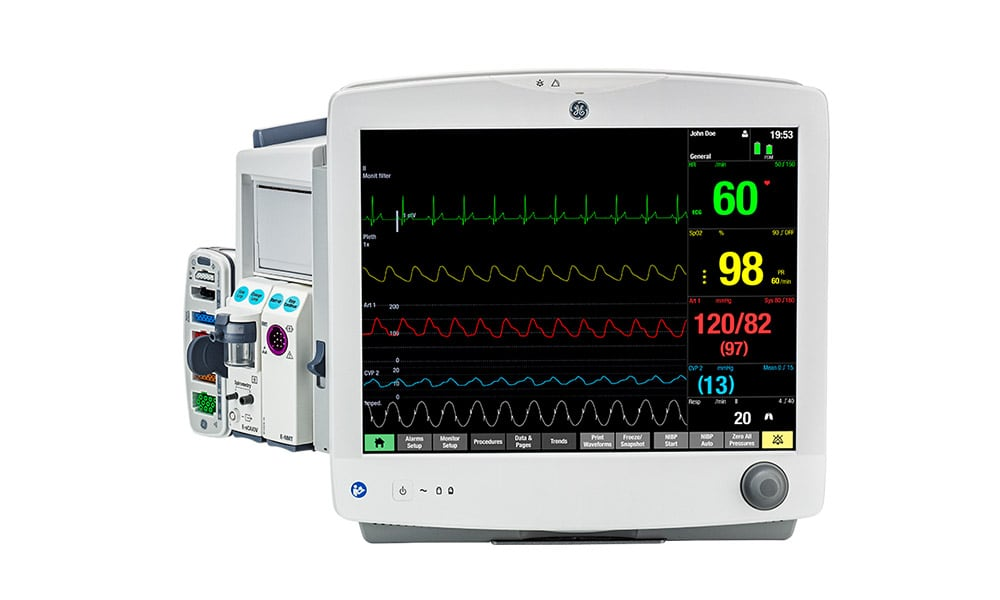
\includegraphics[width=1\textwidth]{ch3/monitor1}
%       \end{minipage}
%       }
%       \quad
%       \subfigure[B650监护界面]{
%       \label{fig:ch5_data}
%       \begin{minipage}[t]{0.5\textwidth}
%       \centering
%       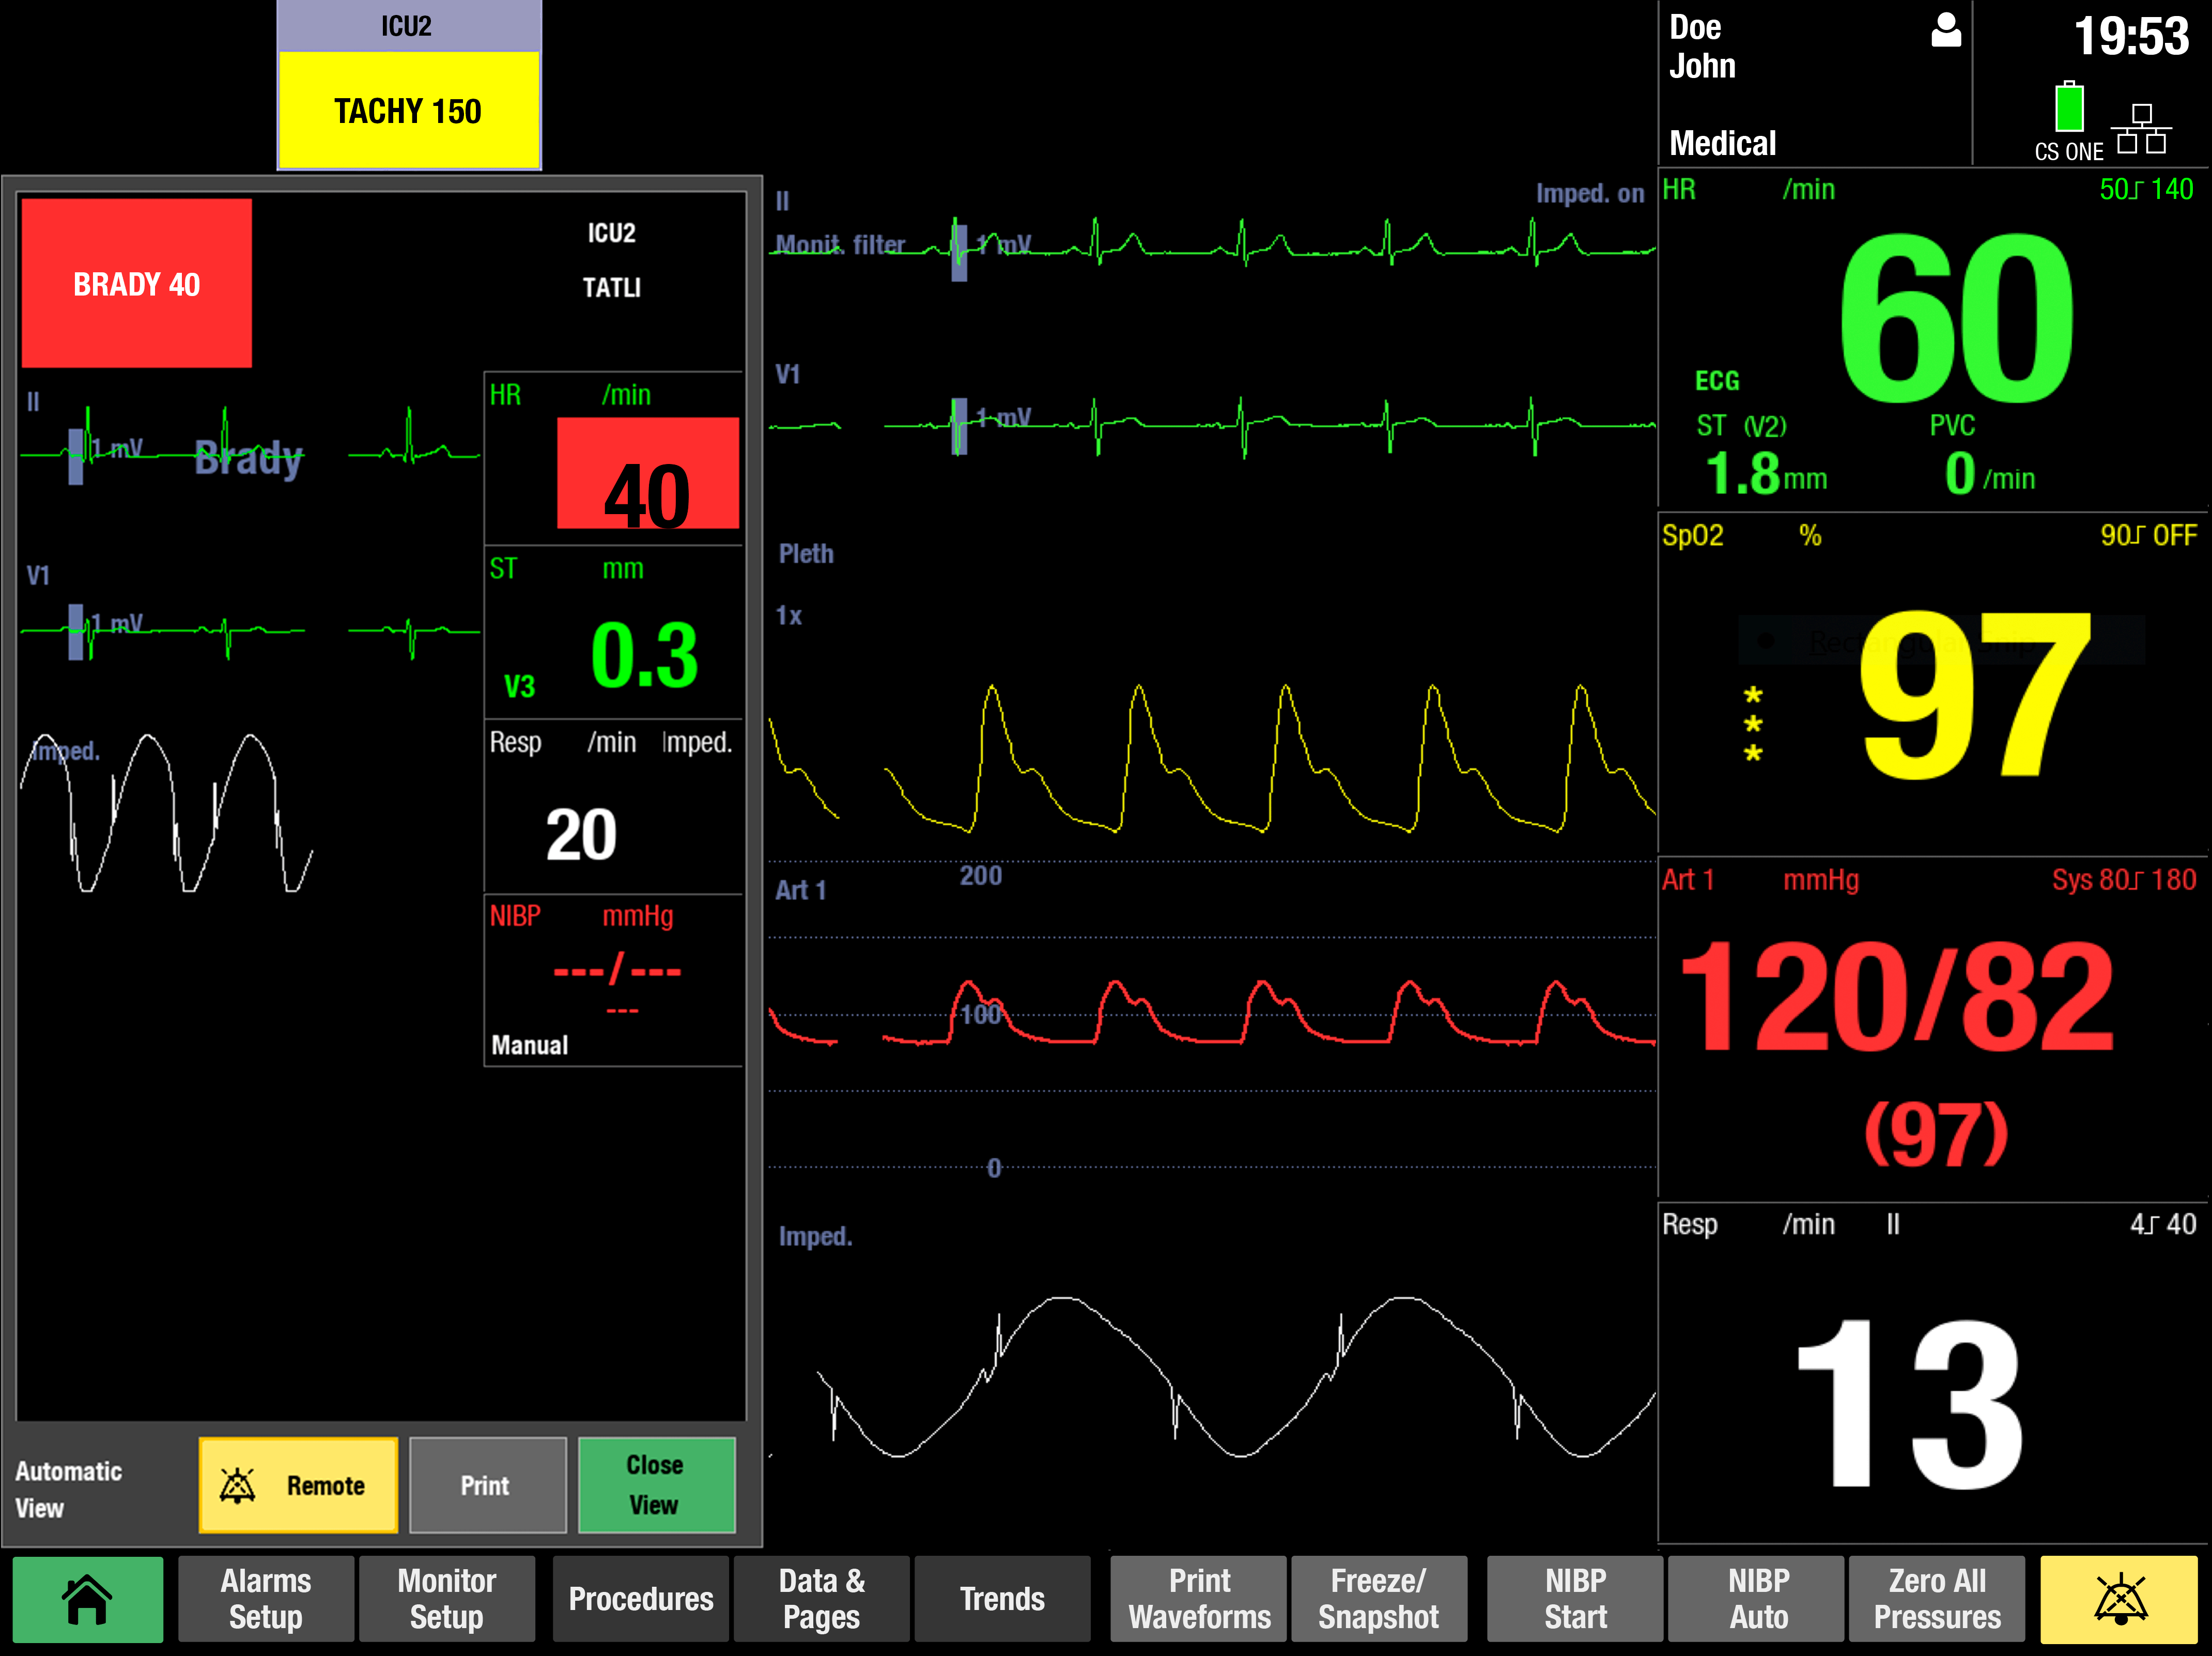
\includegraphics[width=1\textwidth]{ch3/monitor2}
%       \end{minipage}
%       }
%       \caption{\label{fig:monitor}GE Healthcare CARESCAPE B650监护仪}
% \end{figure}
\begin{figure}[htbp]
      \centering
      \subfigure[B650监护仪及其配件]{
      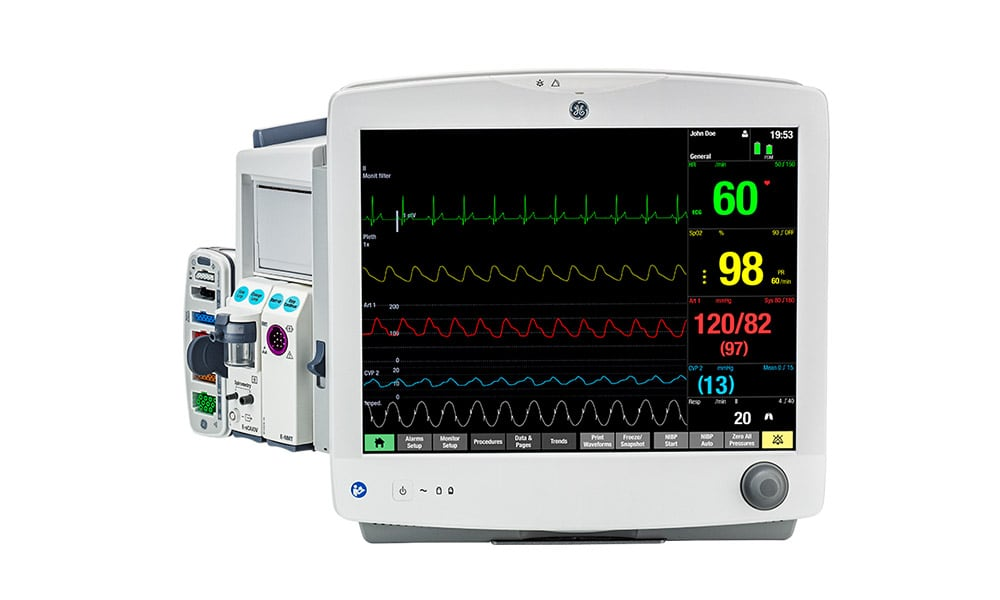
\includegraphics[width=5.5cm]{ch3/monitor1}
      }
      \quad
      \subfigure[B650监护界面]{
      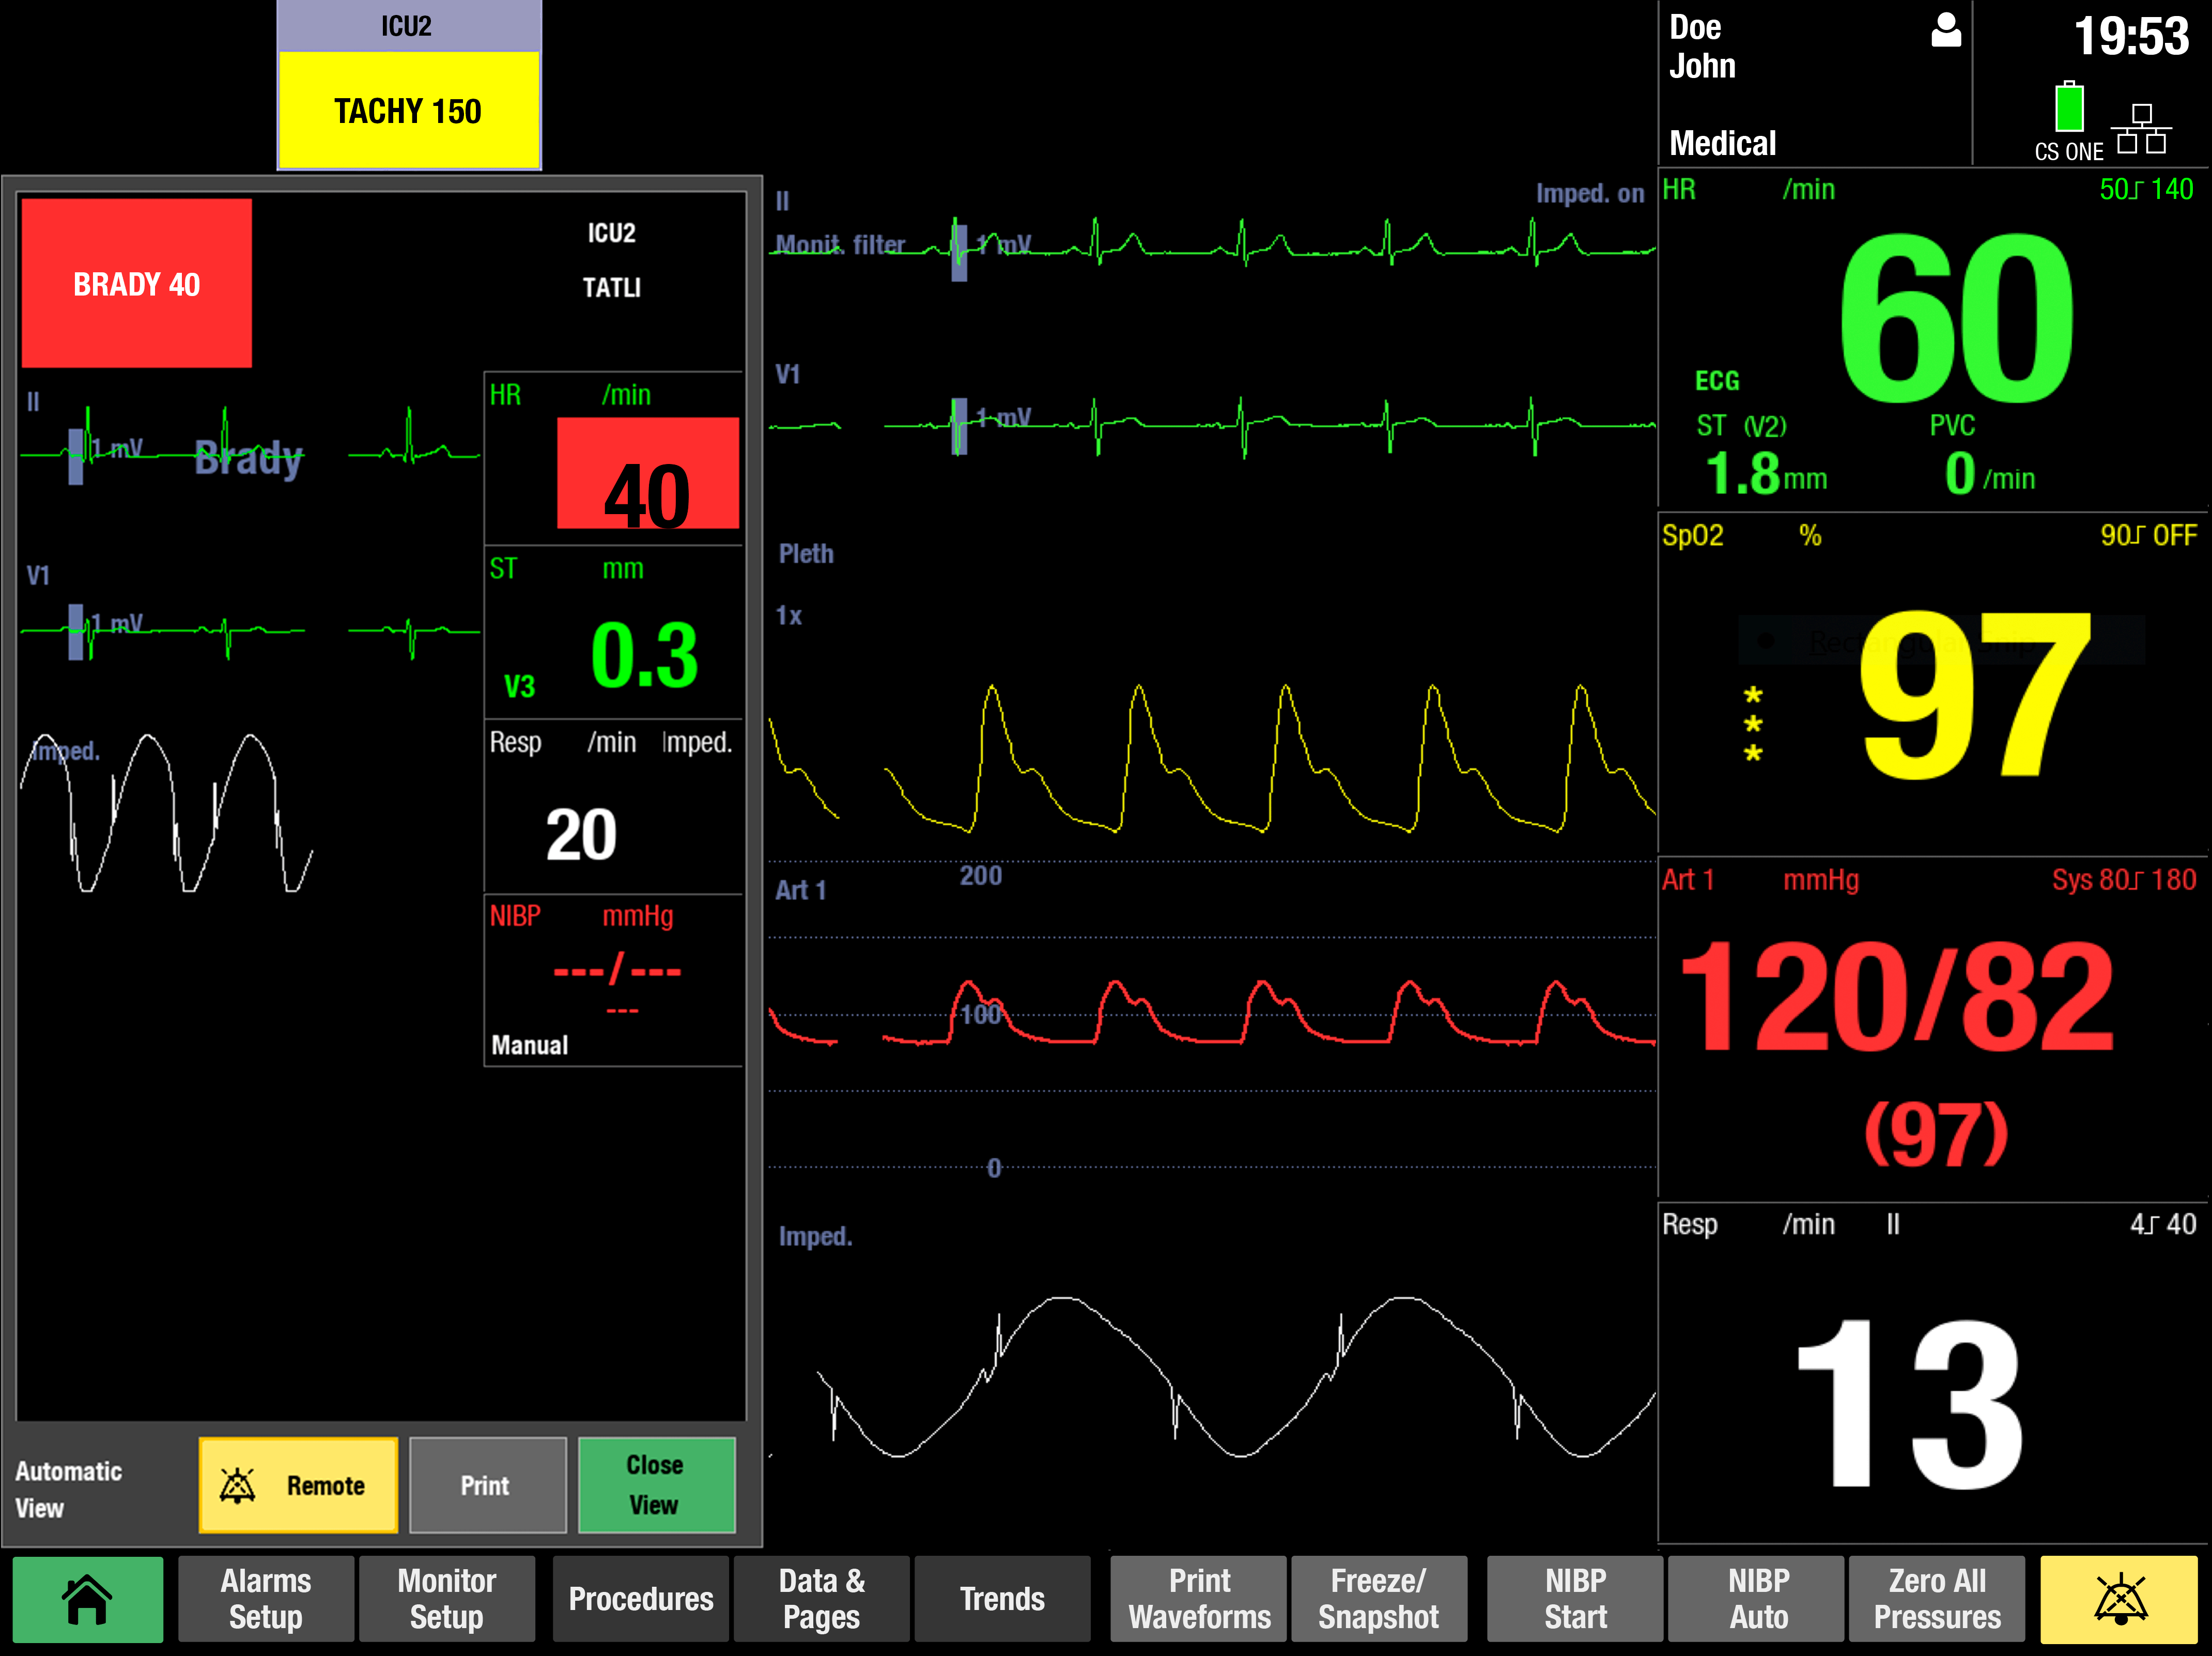
\includegraphics[width=5.5cm]{ch3/monitor2}
      }
      \caption{\label{fig:monitor}GE Healthcare CARESCAPE B650监护仪}
\end{figure}

\subsection{数据采集规范}
如第二章在PPG原理部分所述,本研究最后选取在被试孕妇的左手食指进行使用透射式血氧探头进行采集。若被试孕妇的左手食指有损伤,则将测量部位替换为左手中指,如\autoref{fig:finger}所示。测量时把手指放入指套内部,
指甲与传感器表面有指甲标记的部位正对,指尖触及但不超出指套顶端,确保发光管发出的所有光线全部通过被试的组织。其中,使用的血氧采集探头美国泰科公司旗下的Nellcor DS-100A型血氧传感器。 
\begin{figure}[htbp]
      \centering
      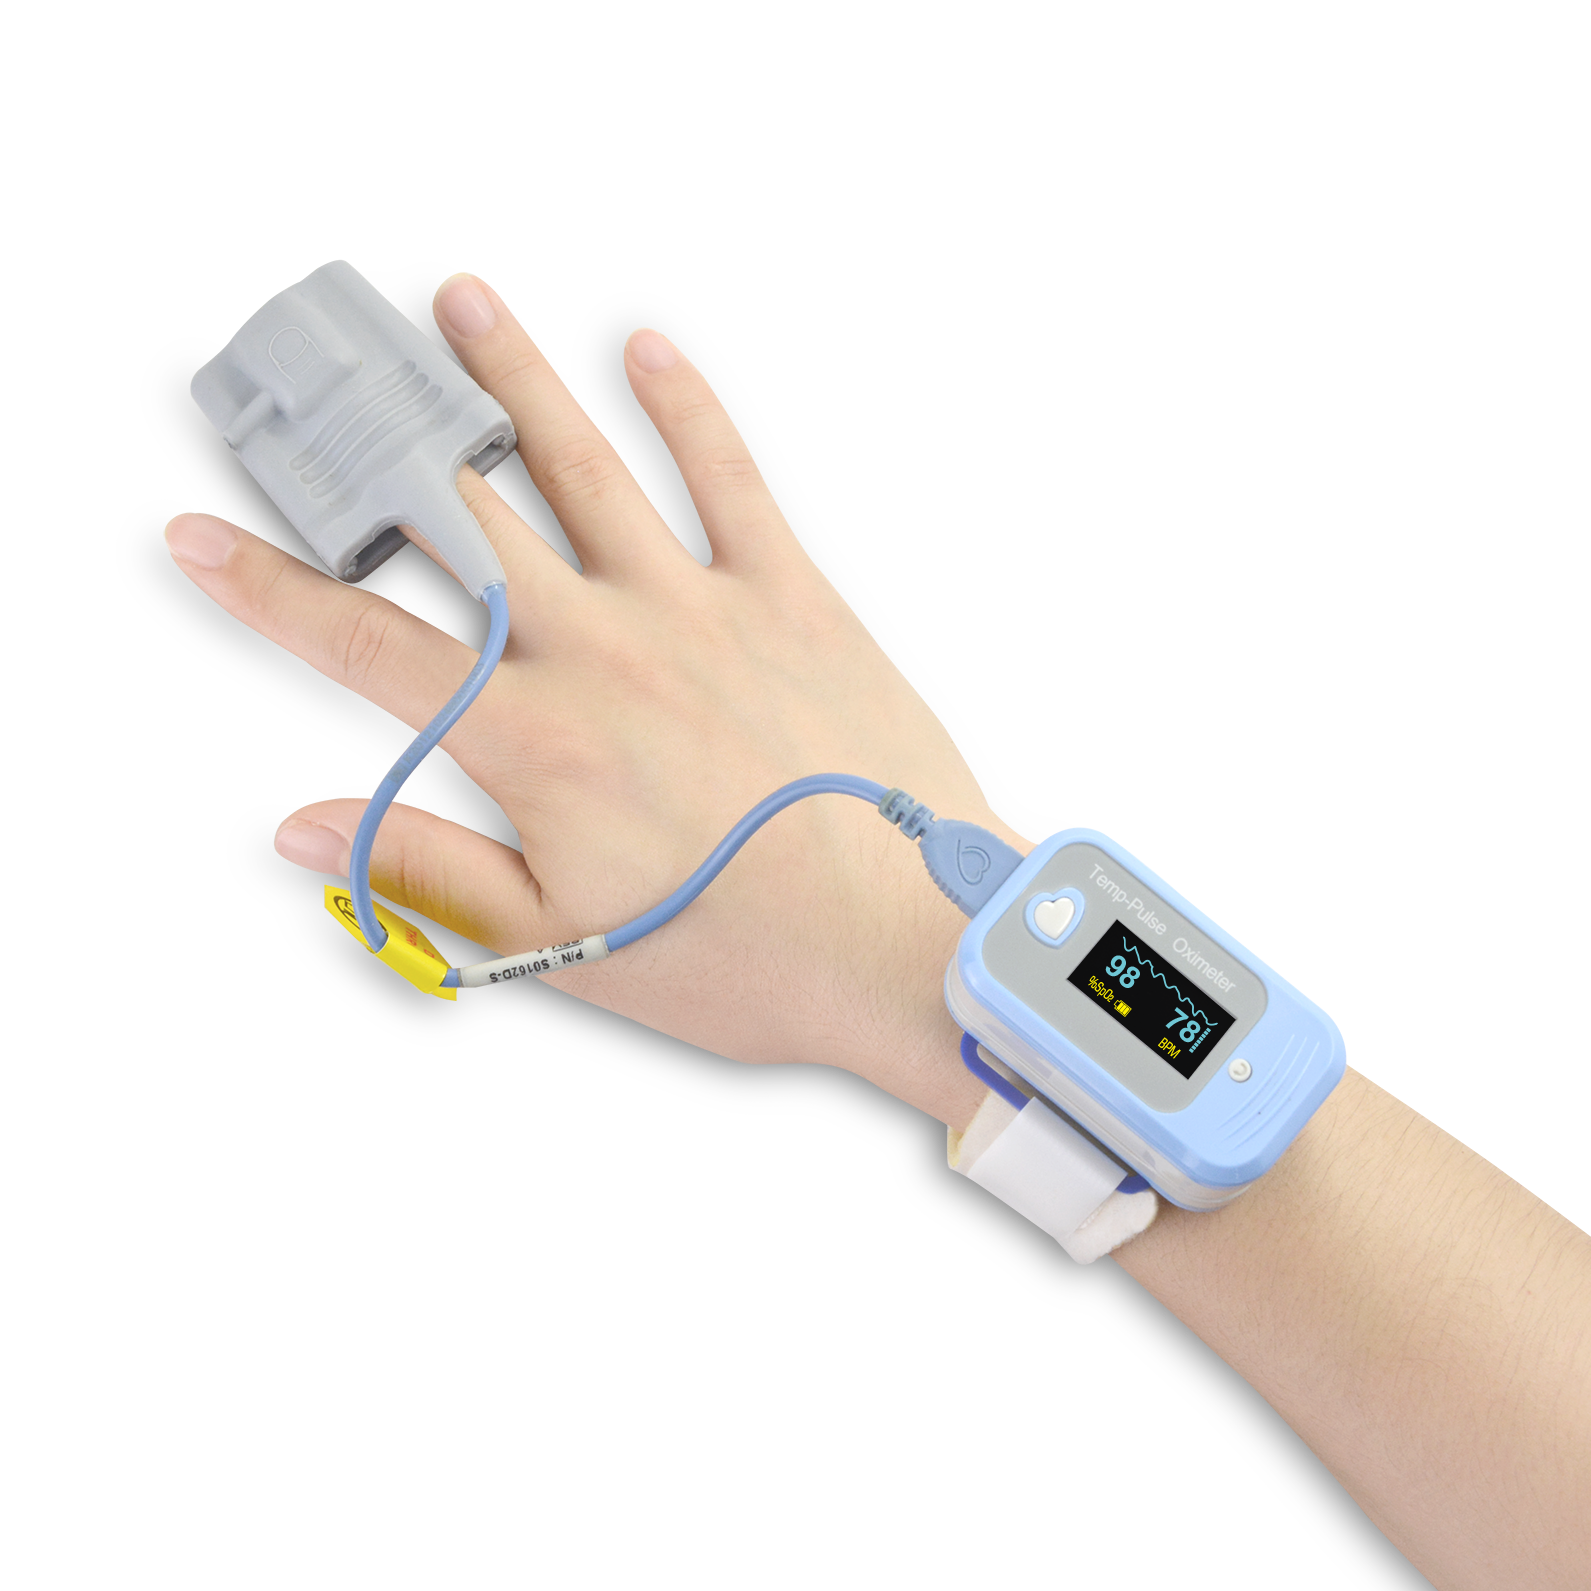
\includegraphics[width=.5\linewidth]{ch3/finger}
      \caption{\label{fig:finger}血氧采集方式示意}
\end{figure}
\subsection{具体实验流程}
被试人员到达数据实验采集现场后,首先登记被试人员包括姓名、年龄、孕产史等一般信息,如\autoref{tab:questionnaire}所示。接着数据采集人员会告知被试人员本研究的研究背景与实验过程。
在征得被试人员同意后,采集人员会按前文操作规范为被试佩戴血氧采集探头\cite{Chen2021}。
与血压采集过程类似\cite{FIGO},被试人员在实验全程需保持坐姿。在被试孕妇休息至少5分钟后,PPG数据开始正式记录,单次采集时长不低于1分钟。
\begin{table}[htbp]
      \centering
      \fontsize{8}{4}
      \caption{指端脉搏波监测孕妇一般资料登记表}
      \label{tab:questionnaire}%
      \begin{tabularx}{\linewidth}{ccccccccccccc}
      % \rowcolor{gray!10}
      \multicolumn{4}{l}{孕妇姓名} & \multicolumn{2}{l}{身高} & \multicolumn{2}{l}{年龄} & \multicolumn{3}{l}{预产期} & \multicolumn{2}{l}{多胎}\\
      \multicolumn{6}{l}{孕产史}   & \multicolumn{5}{l}{本次是否罹患妊娠相关疾病}  & \multicolumn{2}{l}{电话}  \\
      \multicolumn{13}{l}{既往史(有无高血压疾病、糖尿病、肾病、肝病及其他内外科疾病)}  \\
      \Xhline{1.2pt}
      \textbf{孕周} & \textbf{心率} & \textbf{血压} & \textbf{体重} & \textbf{尿蛋白} & \textbf{水肿} & \textbf{转氨酶} & \textbf{胆红素} & 
      \textbf{血小板} & \textbf{凝血功能} & \textbf{胎儿情况} & \textbf{脉搏波采集} & \textbf{备注} \\
      \hline

      &       &       &       &       &       &       &       &       &       &       &       &  \\

      &       &       &       &       &       &       &       &       &       &       &       &  \\
      
      &       &       &       &       &       &       &       &       &       &       &       &  \\

      &       &       &       &       &       &       &       &       &       &       &       &  \\

      &       &       &       &       &       &       &       &       &       &       &       &  \\

      &       &       &       &       &       &       &       &       &       &       &       &  \\

      &       &       &       &       &       &       &       &       &       &       &       &  \\
      \Xhline{1.2pt}
      \end{tabularx}%
\end{table}%  
\subsection{数据导出}
由于GE公司并没有公开B650数据通讯协议,研究无法获得各项生理参数的原始数据信息。经与技术支持沟通,最后B650监护仪可将血氧脉搏波数据以时间——脉搏波相对幅值键值对以CVS的文件格式导出,如\autoref{tab:exporteddata}所示。
其中最终导出的PPG信号采样率为100$Hz$。
\begin{table}[htbp]
      \centering
      \caption{\label{tab:exporteddata}原始导出PPG数据示意}
      \begin{tabularx}{\linewidth}{X<{\centering}X<{\centering}X<{\centering}}
            % \toprule
            \rowcolor{gray!10}
            \textbf{Time,}&\textbf{Pleth(\%),}&\textbf{Event,}\\
            % \midrule
            \rowcolor{gray!10}0402.10:05:47.665178075,&-27,&,\\
            \rowcolor{gray!10}0402.10:05:47.675065560,&-51,&,\\
            \rowcolor{gray!10}0402.10:05:47.684953045,&-82,&,\\
            \rowcolor{gray!10}0402.10:05:47.694840530,&-116,&,\\
            \rowcolor{gray!10}0402.10:05:47.704728015,&-148,&,\\
            \rowcolor{gray!10}0402.10:05:47.714615500,&-176,&,\\
            \rowcolor{gray!10}0402.10:05:47.724502985,&-199,&,\\
            \rowcolor{gray!10}0402.10:05:47.734390470,&-220,&,\\
            \rowcolor{gray!10}…&…&…\\
            % \bottomrule
      \end{tabularx}
\end{table}
\subsection{数据复核}
本研究共采集了81例孕妇的PPG数据段,其中实验组有44例患有PE的孕妇数据,对照组有37条正常妊娠孕妇数据。经复核校验,有x例数据因为采集时间过短、信号质量过低等原因被剔除。
最终,有x例有效PPG数据进入下一阶段的分析研究,其中实验组x例,对照组x例。

\section{常用变量分析方法与性能度量方法}
本研究中需多次衡量变量之间的关系性、评估分类器分类效果及性能对比。本小节将对上述过程中涉及的研究方法及工具指标进行介绍。
\subsection{变量分析方法}
一、相关性分析

相关性分析是指对两个具备相关性的变量元素进行分析,衡量两个变量因素的相关密切程度\cite{Zhang2019}。相关性的元素之间需要存在一定的联系或者概率才可以进行相关性分析。一般可以通过散点图即可直接观察变量之间的联系,如\autoref{fig:relation}所示。
统计学上引入了相关系数$r$以量化表征变量之间的密切程度。常用的相关分析方法有有皮尔逊(Pearson)相关性分析与斯皮尔曼(Spearman)相关性分析,但两者的适用范围有一定差异。斯皮尔曼相关性分析适用于对存在单调性关系的变量进行检测,
而皮尔逊相关性分析适用于对正态分布的变量进行检测。由于本研究中涉及的年龄、血压、心率等参数不满足正态分布,因此,对这些变量的分析均采用了斯皮尔曼相关系数进行衡量。

为计算斯皮尔曼相关系数,首先对长度为$n$的待检二元变量$X$与$Y$按升序排列,得到原始数据在排序后的序次$x$、$y$,特别地,若出现多个数据排序相同,则用这些数据的平均序次统一表征。然后按照\autoref{equ:spearman}计算即可。
\begin{equation}
      \label{equ:spearman}
      r_{s}=1-\frac{6\sum_{i=1}^{n}(x_{i}-y_{i})^2}{n(n^2-1)}
\end{equation}
相关系数$r_{s}$的取值范围为[-1,1],当$r_{s}$>0时,表明两个变量正相关;反之,则两个变量变化趋势相反,呈负相关。$r_{s}$的绝对值反映了两变量之间相关性的强弱,如\autoref{fig:relation}所示。
\begin{figure}[htbp]
      \centering
      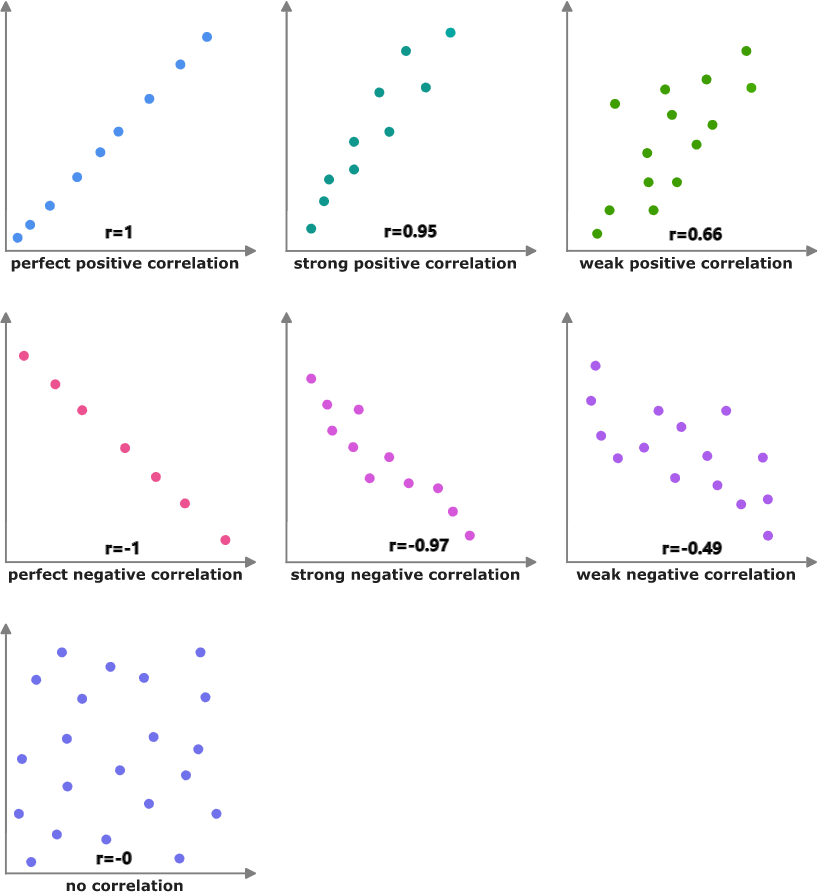
\includegraphics[width=.6\linewidth]{ch3/relation}
      \caption{\label{fig:relation}二元变量之间常见的相关关系}
\end{figure}

二、参数检验与非参数检验

当统计分析方法在理论上要求样本来自特定的总体分布才可对未知总体参数做推断时,此类假设检验方法称为参数检验(parametric test)。而面对总体分布类型未知或分布类型已知,但不对称或变量无法精准测量的数据时,参数检验将无法进行。因此,
另一类不以特定的总体分布为前提、不针对总体分布参数做任何推断的分析方法也发展起来,此类分析方法被统一称为非参数检验(nonparametric test)\cite{Guo2017,Hu2021,Zhang2019}。两大类检验常见的检验方法如所示。

\subsection{性能度量方法}
一、混淆矩阵

混淆矩阵(confusion matrix)是评估分类器分类效果优劣的常用工具\cite{Zhou2016,Aurélien2018}。其总体思路就是分别统计A类别实例被划分成B类别实例的数目。理论上混淆矩阵的行列没有上限,而在实际应用中,二分类任务的混淆矩阵是最常见的。
此时,将样例依据其真实所属类别与分类器预测类别进行组合可得到四种结果:真阳性(true positive,TP)、假阳性(false positive,FP)、真阴性(true negative,TN)及假阴性(false negative,TN),如\autoref{tab:cm}所示。此时显然有
$TP+FP+TN+FN=\text{样例总数}$。
\begin{table}[htbp]
      \centering
      \caption{\label{tab:cm}二分类任务的混淆矩阵}
      \begin{tabular}{ccc}
      \toprule
      \multicolumn{1}{c}{\multirow{2}[4]{*}{\textbf{真实情况}}} & \multicolumn{2}{c}{\textbf{预测结果}} \\
            \cmidrule{2-3}          & 阳性(1) & 阴性(0) \\
      \midrule
      阳性(1) & 真阳性(TP) & 假阴性(FN) \\
      阴性(0) & 假阳性(FP) & 真阴性(TN) \\
      \bottomrule
      \end{tabular}%
\end{table}%

为量化分类器的具体性能,人们在混淆矩阵的基础上衍生定义了一系列数字指标,包括查全率(recall)、查准率(precison)、准确率(accuracy)及特异性(specificity),如\autoref{equ:measures}所示。其中,查全率亦称召回率、
灵敏性(sensitivity)或真阳性率(true positive rate,TPR),查准率亦称精准率,特异性亦称真阴性率。查全率与查准率是应用的最广泛的两个指标\cite{Zhou2016,Aurélien2018}。一般而言,查全率与查准率是对相互矛盾的度量指标,
一个指标性能的提高意味着另一个指标性能的下降。通常只有在简单分类任务中,
才能同时获得较高的查准率与查全率。这称为精度-召回率权衡。为评估查全率与查准率均不相等的分类器性能,人们进一步定义了$F_1\text{分数}$,如\autoref{equ:f1}所示。$F_1\text{分数}$是召回率与精准率的谐波均值。
召回率与精准率相近的分类器易获得更高的$F_1\text{分数}$。
\begin{equation}
      \label{equ:measures}
      \left \{
      \begin{aligned}
            Recall      &=\frac{TP}{TP+FN}         \\
            Precison    &=\frac{TP}{TP+FP}          \\
            Accuracy    &=\frac{TP+TN}{TP+FP+TN+FN} \\
            Specificity &=\frac{TN}{TN+FP}       \\
      \end{aligned}
      \right.
\end{equation}
\begin{equation}
      \label{equ:f1}
      F_1=\frac{2}{\frac{1}{Precison}+\frac{1}{Recall}}=\frac{2\cdot Precison\cdot Recall}{Precison+Recall}=\frac{TP}{TP+\frac{FN+FP}{2}}
\end{equation}

在评估分类器性能时需要根据场景,从\autoref{equ:measures}与\autoref{equ:f1}中灵活选取恰当的评价指标。

二、ROC曲线、AUC与约登指数

受试者工作特征(Receiver Operating Characteristic,ROC)曲线是另一种常用于二分类问题的分析工具。ROC绘制的是真阳性率和假阳性率(false positive rate,FPR)之间的变化关系,其中
\begin{equation}
      \label{equ:fpr}
      FPR=\frac{TN}{TN+FP}=1-Specificity
\end{equation}
因此,ROC曲线也被称为灵敏度与1-特异性曲线。绘制曲线时,以分类器的预测结果对样例进行升序排列,依次将样本作为阳性进行预测,计算对应的TPR与FPR后,可得一坐标点$({FPR}_i,{TPR}_i)$,最后将所有坐标点连线即可,如所示。
其中,虚线表示纯随机分类器的ROC曲线,理想性能的分类器应无限逼近左上角(即$\text{坐标点}(0,1)$)。

在衡量多个分类器性能优劣时,常将分类器对应的ROC曲线下面积作为判据,即为AUC(Area Under Curve)。纯随机分类器ROC的AUC数值为0.5,而理想分类器ROC的AUC数值为1,如所示。

此外,约登指数(Youden Index)也是用来评价分类器效果的一个指标。若在评估分类器性能时,给予将分类器假阴性和假阳性以相同权重,即可应用约登指数
\begin{equation}
      \label{equ:yi}
      \begin{aligned}
            YI&=Sensitivity-(1-Specificity)\\
            &=Sensitivity+Specificity-1
      \end{aligned}
\end{equation}
一般认为,当YI取值最大时,此时对应的分类阈值为最佳阈值\cite{cwl}。

\section{人口统计学特征分析}
在本研究中,由于年龄、血压、心率等待检参数样本量较小、具体分布未知,因此,对这些变量的分析均采用了非参数检验。
\section{小结}
本章对实验数据进行了详细的说明,从实验具体流程、到具体采集设备等在内对采集方案进行了详细的说明。此外,本章也同时对被试孕妇的人口统计学特征进行了研究分析,结果表明,被试人群中,排除了等因素的干扰,
符合数据筛选标准,可以用于后续分析研究。  